\documentclass{beamer}
\usepackage[utf8]{inputenc}
\usepackage[slovak]{babel}
\usepackage{hyperref}
\usepackage{algorithmic}
\usetheme{Boadilla}
\setbeamertemplate{footline}[page number]

\title[Quicksort]{Radiace algoritmy - Quicksort}
\institute
{
  Fakulta informačných technológií\\
  Vysoké učení technické v Brne
}
\author[Adam Zvara]{Adam Zvara, xzvara01(@vutbr.cz)}
\date{\today}

% display frame counter
\setbeamertemplate{page number in head/foot}[totalframenumber]
\beamertemplatenavigationsymbolsempty

\newcommand{\cmnt}[1]{\textcolor{teal}{#1}}

\begin{document}

\frame[plain]{\titlepage}

\begin{frame}{Obsah}
  \setbeamertemplate{section in toc}[sections numbered]
  \tableofcontents
\end{frame}

\section{Radiace algoritmy}
\begin{frame}{Radiace algoritmy}
  \begin{block}{Definícia}
    \structure{Radenie} \cite{IALSorting} je usporiadanie položiek podľa relácie lineárneho usporiadania nad kľúčmi
  \end{block}
  \begin{itemize}
    \item Riadenie je často základom iných algoritmov
    \item \structure{Kanonizácia} údajov
    \item Výstup zrozumiteľný pre človeka
  \end{itemize}
\end{frame}

\section{Radiaci algoritmus quicksort}
\begin{frame}{Radiaci algoritmus quicksort}
  \begin{itemize}
    \item Založený na machanizme \alert{rozdelenia} (partition)
      \begin{itemize}
        \item Výber mediánu (v praxi \structure{pseudomedián})
        \item Vytvorenie 2 indexov na prechádzanie poľa zľava a sprava 
        \item Zľava hľadáme prvok väčší alebo rovný mediánu, sprava menší alebo rovný mediánu
        \item Nájdené prvky medzi sebou vymeníme
        \item Proces ukončíme v prípade že sa indexy prekrížia
    \end{itemize}
    \item Mechanizmus rozdelenia voláme nad nezoradeným poľom \structure{rekurzívne}
  \end{itemize}
\end{frame}

\section{Mechanizmus partition - pseudokód}
\begin{frame}{Mechanizmus partition - pseudokód \cite{QuicksortPseudo}}
    \vspace{-0.7em}
    \footnotesize
    \begin{algorithmic}
      \STATE\hspace{-\algorithmicindent}{\textbf{\color{blue}partition} (array, left, right)}
      \STATE{$i \leftarrow left$}
      \STATE{$i \leftarrow right$}
      \STATE{$PM \leftarrow A[\,(i+j) div 2\,]$} \hfill \cmnt{// nastavenie pseudomediánu}
      \REPEAT
      \WHILE{$array[\,i\,] < PM$}
        \STATE{$i \leftarrow i + 1$}  \hfill \cmnt{// prvý prvok zľava, ktorý je väčší než pseudomedián}
      \ENDWHILE
      \WHILE{$array[\,i\,] > PM$}
        \STATE{$j \leftarrow j - 1$} \hfill \cmnt{// prvý prvok sprava, ktorý je menší než pseudomedián}
      \ENDWHILE
      \IF{$i \leq j$}
        \STATE{$array[\,i\,] \longleftrightarrow array[\,j\,]$} \hfill \cmnt{// výmena nájdených prvkov}
        \STATE{$i \leftarrow i + 1$}
        \STATE{$j \leftarrow j - 1$}
      \ENDIF
      \UNTIL{$i > j$} \hfill \cmnt{// koniec keď sa indexy prekrížia}
      \RETURN{$(i,j)$} 
      \end{algorithmic}
    \label{alg:partition}
\end{frame}

\section{Quicksort - pseudokód}
\begin{frame}{Quicksort - pseudokód \cite{QuicksortPseudo}}
    \footnotesize
    \begin{algorithmic}
      \STATE\hspace{-\algorithmicindent}{\textbf{\color{blue}quicksort} (array, left, right)}\\
      \cmnt{// Pri volaní má left hodnotu 0 a right hodnotu ARRAY\_LENGTH - 1}\\
      \STATE{$i, j \leftarrow partition(array, left, right)$}
      \IF{$left < j$}
        \STATE{$quicksort(array, left, j)$}
      \ENDIF
      \IF{$i < right$}
        \STATE{$quicksort(array, i, right)$}
      \ENDIF
      \end{algorithmic}
    \label{alg:quicksort}
\end{frame}

\begin{frame}{Quicksort - príklad}
  \begin{center}
    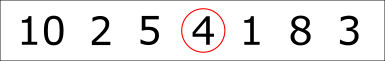
\includegraphics[scale=0.6]{img/quicksort_p1.png}
    \pause
    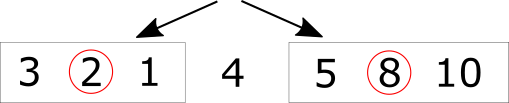
\includegraphics[scale=0.6]{img/quicksort_p2.png}
    \pause
    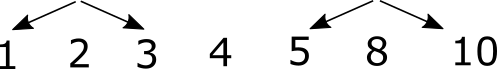
\includegraphics[scale=0.6]{img/quicksort_p3.png}
  \end{center}
\end{frame}

\section{Ohodnotenie algoritmu}
\begin{frame}{Ohodnotenie algoritmu}
  \begin{itemize}
    \item Jeden z najrýchlejších algoritmov na radenie polí
    \item \alert{Nestabilný}, neprirodzený
    \item \textbf{\structure{Linearitmická}} časová zložitosť pre vhodný pseudomedián
    \begin{itemize}
        \item Pre ideálny pseudomedián každé volanie rozdelí pole na 2 rovnaké časti $O(\log n)$
        \item Pre každé volanie musíme prejsť $N$ vstupov $O(N)$
    \end{itemize}
    \item Najhoršia časová zložitosť je \alert{\textbf{kvadratická}}
    \begin{itemize}
        \item Nevhodný pseudomedián rozdelí pri každom volaní pole na 2 nerovnomerné časti $O(N)$
        \item Pre každé volanie musíme prejsť $N$ vstupov $O(N)$
    \end{itemize}
  \end{itemize}
\end{frame}

\section{Použité zdroje}
\begin{frame}{Použité zdroje}
  \begin{thebibliography}{9}
    \bibitem{IALSorting} 
    Honzík J. M., Burgetová I., Křena B., \emph{Algoritmy - IAL - 7. prednáška} [Online], Brno FIT VUT, 2020. [prístup 24.04.2022] Dostupné na: \href{https://wis.fit.vutbr.cz/FIT/st/cfs.php.cs?file=\%2Fcourse\%2FIAL-IT\%2Flectures\%2FPred-07_2021_final.pdf&cid=14603}{\texttt{https://wis.fit.vutbr.cz/FIT/st/cfs.php.cs}}
    
    \bibitem{QuicksortPseudo} 
    Honzík J. M., Burgetová I., Křena B., \emph{Algoritmy - IAL - 8. prednáška} [Online], Brno FIT VUT, 2020. [prístup 24.04.2022] Dostupné na: \href{https://wis.fit.vutbr.cz/FIT/st/cfs.php.cs?file=\%2Fcourse\%2FIAL-IT\%2Flectures\%2FPred-08_2021_final.pdf&cid=14603}{\texttt{https://wis.fit.vutbr.cz/FIT/st/cfs.php.cs}}

\end{thebibliography}
\end{frame}

\end{document}
